\chapter{文献综述}
    
% 当前,新一轮科技革命和产业变革加速发展,新一代信息技术正在与工业生产 深度融合,自动化、信息化、智能化已经成为全球工业制造发展的重要方向。
% 2020年李克强总理发布的《政府工作报告》中,明确提出“推动制造业升级”、“推进智能制造”的要求。如何工业生产利用智能化技术,将,

% 为了实现工业4.0、工业互联网、数字孪生等伟大技术愿景,其中


% 复杂工业系统的控制与优化是典型的交叉学科,计算机、自动化、控制工程、仪器仪表等。
% 伴随着人工智能与数据科学的发展,数据驱动的复杂系统建模与控制优化技术逐渐应用。
% 现存问题:如何合理地将深度学习与工业过程特性深度融合,同时有效地指导系统优化并实现智能控制,对此部分的研究迫在眉睫。
% 本文面向具有长时延特性、周期多阶段性、非确定性的三类复杂工业系统,提出一套基于ODE-Net的动态系统建模方法,并在构建模型的基础上,提出了基于有模型强化学习理论的控制优化方法,并成功应用于工业实践。实现了xxx目标,为数据驱动的工业系统建模及控制优化提供了新的研究思路。
\section{动态系统辨识及有模型控制的起源与发展}
\label{sec:2_1}
% 基于数据驱动的复杂工业系统预测建模方法可以分成两大类:离散时间(Discrete Time, DT)系统建模和连续时间系统建模。

从机器学习的视角来看,系统建模本质上是一种有监督学习问题\cite{jordan1992forward}。本节主要从模型参数估计方法以及基于模型的优化控制两方面对动态系统辨识及有模型控制进行简要介绍。

对于动态模型,假定其系统状态表示为$s_t$,系统输入为$a_t$,给定批量的状态转移数据,我们可以学习前向模型$\left(s_t, a_t\right) \rightarrow s_{t+1}$,即给定当前状态和选择的动作,预测下一个状态。
利用学习得到的前向模型可以辅助实现系统的控制优化,比如如模型强化学习、模型预测控制等\cite{moerland2020model}。
基于有监督学习的前向模型辨识方法可以划分为参数化方法和非参数化方法两种,
进一步按照模型是否有随机性分类分为精确模型和近似模型。

非参数化的精确建模方法采用回放池\cite{lin1992memory}方法存储系统的历史轨迹,并将前向预测过程转化为检索问题。
对于非参数的近似建模方法,比较常见的是高斯过程模型\cite{deisenroth2011pilco,deisenroth2011pilco},通过利用历史部分状态-动作点,可以外推预测某一新给定状态-动作点的高斯分布$p\left(f^* \mid \boldsymbol{x}^*, \boldsymbol{f}, \boldsymbol{X}\right)=\mathcal{N}\left(f^* \mid \mu, \sigma^2\right)$,
其中$\boldsymbol{X}$代表完整数据集,$\boldsymbol{f}$代表$\boldsymbol{X}$上的观测。$\boldsymbol{x}^*=[s_t,a_t]$代表
给定当前时刻状态和控制输入下,系统的预测结果。
% 询问的新的输入
该方法预测出的高斯分布中的方差$\sigma^2$能够对系统演化的非确定性给出度量。

相比于非参数化方法,参数化方法的参数数量与观测数据集的大小是独立的
。为了避免过高的空间复杂度以及预测计算量,参数化方法的应用更为广泛。参数化的精确建模方法也称为表格方法,对于每一种可能的转移维护独立的转移概率。如随机马尔可夫决策过程(Markov Decision Process,MDP),基于表格的最大似然模型能够统计每一种转移的概率:
\begin{equation}
    T\left(s^{\prime} \mid s, a\right)=\frac{n\left(s, a, s^{\prime}\right)}{\sum_{s^{\prime}} n\left(s, a, s^{\prime}\right)}
\end{equation}
% where $T$ denotes the approximation of the true dynamics $\mathcal{T}$, and $n\left(s, a, s^{\prime}\right)$ denotes the number of times we observed $s^{\prime}$ after taking action $a$ in state $s$. This approach
$T$代表真实系统$\mathcal{\mathcal { T }}$的近似,
$n\left(s, a, s^{\prime}\right)$ 代表在数据集中状态$s$下执行动作 $a$产生状态$s^{\prime}$的频次。表格法作为最简单的系统建模方法,随着状态集$\mathcal{S}$的增大,表格的大小呈指数增加,因此难以扩展到高维问题。

另一种参数化建模的方式是对转移函数进行参数近似,在相似状态之间实现信息的泛化,以充分降低对于存储以及数据量的需求。
由于该方法适用面广、空间占用少、计算速度快,
函数近似也因此成为解决连续空间以及高维动态系统建模问题的主流方法。
理论上,可以使用任意参数近似方法学习模型,如线性回归\cite{silver2008sample},动态贝叶斯网络、随机森林、最近邻搜索、神经网络\cite{werbos1989neural}等。

近十年来,深度学习逐渐成为解决复杂函数近似问题的主流方法。因为复杂动态系统往往具备典型的高维输入输出空间以及非线性特性,基于深度神经网络的动态系统辨识模型也逐渐受到广泛关注。
利用神经网络的前向传播过程模型可以模拟系统的动态过程\cite{temeng1995model, tan1996nonlinear}。
循环神经网络(Recurrent neural network, RNN)作为一种拥有马尔科夫特性的网络模型,与动态系统极为类似,且因为隐状态的存在,RNN能够很好地处理长时依赖问题以及长期预测问题,因此在系统建模领域被广泛应用\cite{delgado1995dynamic, zamarreno1998state}。
本文的研究重点也限定在参数化的、函数近似的、基于深度学习的系统动态建模方法中,探究面向不同类型动态系统的网络设计以及学习方法。


% TODO 没写控制

\section{连续时间系统辨识}

% 依托于近年来机器学习、强化学习\cite{sutton2018reinforcement}、深度学习\cite{lecun2015deep}\cite{duan2016}、时间序列分析技术\cite{shumway2000time}的发展与普及,
在过去的几十年间,数字计算机技术发展迅猛。
从离散时间(Discrete-time, DT)角度进行系统建模的研究方向涌现出了诸多成果,领域发展相对较为成熟,其原因与数字计算机将信息离散化的思想密不可分。
相比而言,连续时间(Continuous-time, CT)系统作为最早的系统辨识研究范式,近年来其相关理论体系研究较为滞后。
但是对比离散时间模型,从连续时间域角度进行系统建模在某些情况下具有较大优势:
\begin{itemize}
\setlength{\itemsep}{0pt}
\setlength{\parsep}{0pt}
\setlength{\parskip}{0pt}
\setlength{\topsep}{0pt}
\setlength{\partopsep}{0pt}
\item	\textbf{对于物理属性的兼容性}:大部分的物理现象都服从连续时间设定,如化学、动力学、热力学等典型场景都可以利用微分方程进行表述,因此利用连续时间模型对物理系统进行建模可以更好地匹配客观世界物理规律,且增加模型的可解释性。
\item	\textbf{对于先验知识的表示}:以动力学系统为例,动量、位移、质量之间的相关性可以在连续时间系统下非常容易地表示出来,而对于表示此类先验特性会更加复杂。因此连续时间模型能够更有效地利用系统先验知识,降低模型求解的自由度。
\item \textbf{潜在的数据滤波}:一般的系统辨识过程需要执行特定的预过滤策略以消除数据中的噪音。而连续时间系统建模方法本质上包含了数据预过滤过程,避免了预处理过程对于原始数据特性的破坏。
\item \textbf{非均匀的数据采样}:当数据采样间隔不均匀时,离散时间方法无法使用,但是连续时间辨识方法能够有效解决非均匀采样问题。
\item \textbf{连续时间系统与离散时间系统的相互转换}:对于连续时间系统可以通过变更采样率的方法获得任意时间间隔的离散时间系统。而对于离散时间辨识系统,当预测步长与下游应用所需的时间间隔不一致时,模型无法适用。
\item \textbf{离散时间模型在高采样率下存在精确性问题}:当数据采样率较高时,系统在相邻时刻间的状态变化较小,不适宜的DT模型难以从微小的状态变化中学习系统动态,导致模型的开环预测结果存在精度差、鲁棒性低的问题。连续时间模型本质上是学习连续时间域下的微分方程,采样率越高,轨迹越完备,学习效果越好。
\item \textbf{刚体性系统建模}:当系统同时存在快过程和慢过程时,离散采样的间隔选取不当很容易造成快过程或慢过程其中一类统计性质的丢失,对离散时间系统处理造成较大阻碍。而连续时间模型能够从频域角度对不同频率的演化过程进行协同建模。
\end{itemize}
对于复杂工业系统,上述七大特性或需求是时常出现的。
因此,最早的系统辨识方法研究也大多是围绕连续时间系统展开的。
% \subsection{基于数据驱动的复杂工业系统建模及控制}
系统通常是由表征系统输入输出关系的数学模型描述的,这个模型有其特定的结构和参数。以代数方程表示的系统称为静态系统,
考虑最简单的形式,系统的连续时间模型可以建模为常系数微分方程:
\begin{equation}
\frac{\mathrm{d}^{n} y(t)}{\mathrm{d} t^{n}}+a_{1} \frac{\mathrm{d}^{n-1} y(t)}{\mathrm{d} t^{n-1}}+\cdots+a_{n} y(t)=b_{0} \frac{\mathrm{d}^{m} u(t)}{\mathrm{d} t^{m}}+\cdots+b_{m} u(t)+v(t)
\label{equ:linear_ct_dyn}
\end{equation}
$\frac{d^{i} x(t)}{d t^{i}}$代表信号$x(t)$对时间的$i$阶导数,$v(t)$是常数项。该式表示了在任一时刻系统输出$y(t)$对时间的各阶导数与输入量$u(t)$对时间的各阶导数之间存在的线性关系。

一般地,对于任意阶数的线性齐次微分方程可以转化为状态空间模型的形式:
% 对上式进行简化,仅考虑状态的最高一阶导数与输入量的零阶导数,并引入非线性成分,得到:
\begin{equation}
    \left\{
    \begin{aligned}
\dot {\boldsymbol h}(t)&=f(\boldsymbol h(t), \boldsymbol{u}(t))\\
\boldsymbol y(t)&= C \boldsymbol h(t)
    \end{aligned}
    \right.
\end{equation}
$f$为系统动态,$C$为投影矩阵,$\boldsymbol h(t)$代表系统的隐空间状态。
% 动力学理论驱动的微分方程模型已经普遍存在于经典数学建模中。
对于线性系统\equref{equ:linear_ct_dyn},$f$可以表示为线性函数。然而,对于许多客观世界存在的复杂动力学系统,
动态$f$时常表现为具有较强非线性特性的某一未知函数,
想要基于第一性原理近似推导出的系统的方程结构是极其困难,
% 这也导致理论模型在大部分情况下无法准确描述的行为。
这也导致传统的系统参数辨识方法难以适用,
制约了控制优化理论在复杂工业系统中的应用。
因此,该领域亟需一种先进的系统建模或辨识方案,能够在模型参数结构未知的情况下,从连续时间域角度对系统进行高精度的黑盒辨识。

% 为了解决该问题,前人通过将机理模型结构与高性能函数逼近器\cite{funahashi1993approximation}相结合,有效缩小了理论模型与观察数据之间的差距,提升了对函数$f$建模的准确性。这项工作也是最早地将连续时间神经网络与动态系统问题
% \subsection{基于编解码结构的系统预测}
% 当系统具有较大时延,即高时滞特性下,模型需要考虑历史数据对未来系统变化的影响。Felipe 等\cite{demeester2020system}利用带有Attention组件的Encoder-Decoder模型对一种名为膏体浓密机系统进行建模识别,Yuan等\cite{Yuan2020}采用一种更复杂的名为双注意力循环神经网络(Dual Attention Recurrent Neural Network, DARNN)的RNN网络对工业系统进行建模,两种方法都考虑了系统变量之间的长期依赖性,利用循环神经网络加Attention机制的强大编码能力,对历史数据、不同维度数据进行信息编码,来辅助输出量的预测,并且利用预测误差对编码器部分进行训练调整。然而两种方法都是针对离散时间系统设计的,不适用于连续时间系统建模问题。
% \section{深度微分方程网络}
% \subsection{深度微分方程网络总描述}
% \subsection{微分方程网络概述}

\section{微分方程网络在复杂系统建模中的应用}
发表自神经信息处理会议2018(Neural Information Processing,NIPS 2018)的一篇开创性文章\cite{chen2018neural}提出了一种神经常微分方程网络,其采用神经网络参数化微分方程的向量域\cite{kidger2021}:
\begin{equation}
y(0)=y_0 \quad \frac{\mathrm{d} y}{\mathrm{~d} t}(t)=f_\theta(t, y(t))
\end{equation}
其中$f_\theta: \mathbb{R} \times \mathbb{R}^{d_1 \times \cdots \times d_k} \rightarrow \mathbb{R}^{d_1 \times \cdots \times d_k}$代表标准的神经网络结构,$\theta$代表可学习的神经网络参数。
$y:[0, T] \rightarrow \mathbb{R}^{d_1 \times \cdots \times d_k}$代表微分方程的解。
使用神经微分方程的核心目的是将微分方程求解过程作为可微算子嵌入在计算图,利用联合敏感度定理\cite{chen2018neural}计算损失函数对$\theta$以及连续时间隐状态$y(t)$的梯度,进而训练微分方程网络中的参数。
% 图\ref{fig:neural_ode}给出了一个简单神经常微分方程的计算图。
% \begin{figure}[h]
%     \centering
%     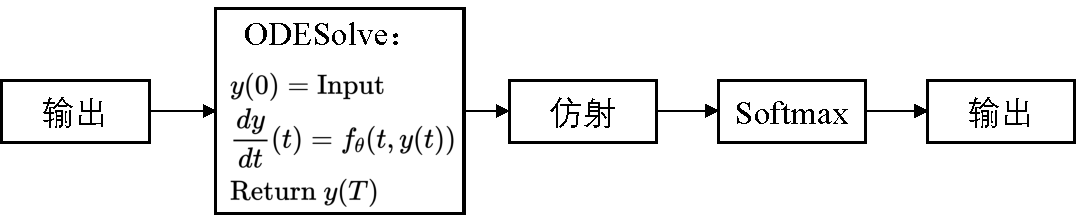
\includegraphics[width=0.9\linewidth]{figures/chapter1/simple_ode.pdf}
%     \caption{神经常微分方程的计算图}
%     \label{fig:neural_ode}
% \end{figure}

ODE-Net的主要应用包括作为Res-Net的替代、时序过程建模以及可逆正则化流\cite{Grathwohl2019}。本文主要围绕ODE-Net在时间序列建模及系统辨识中的应用展开研究。
ODE-Net将\ref{sec:2_1}节所述的连续时间模型的优势引入到基于深度学习的时间序列模型中,因此开辟了时间序列分析、动态系统建模研究的新思路。
% 接下来本节将简单介绍几种常见的微分方程网络及其应用。

以建模捕食者物种和被捕食物种之间相互作用的Lotka-Volterra模型为例,可以采用带有未知参数的常微分方程表示:
\begin{equation}
    \begin{gathered}
    \frac{\mathrm{d} x}{\mathrm{~d} t}(t)=\alpha x(t)-\beta x(t) y(t) \in \mathbb{R} \\
    \frac{\mathrm{d} y}{\mathrm{~d} t}(t)=-\gamma x(t)+\delta x(t) y(t) \in \mathbb{R} .
    \end{gathered}
    \label{equ:2_ode}
\end{equation}

其中$x(t)$和$y(t)$分别表示被捕食者和捕食者的种群大小。在每个时间t,右侧是理论经验公式,表示物种之间的交互作用。
在一般情况下,尽管上述经验公式中的模型参数可以通过经典系统辨识方法进行有效估计,
% 但是模型结构本身过于理想化,难以保证精确性。
但是模型方程往往是经过一定程度的问题简化得到的,
模型的预测值相对于实际观测数据会有明显差距。
为了纠正该偏差,可以在模型中引入神经网络$f_\theta, g_\theta: \mathbb{R}^2 \rightarrow \mathbb{R}$,并构建如下模型:
\begin{equation}
    \begin{aligned}
    \frac{\mathrm{d} x}{\mathrm{~d} t}(t) &=\alpha x(t)-\beta x(t) y(t)+f_\theta(x(t), y(t)) \in \mathbb{R} \\
    \frac{\mathrm{d} y}{\mathrm{~d} t}(t) &=-\gamma x(t)+\delta x(t) y(t)+g_\theta(x(t), y(t)) \in \mathbb{R}
    \end{aligned}
    \label{equ:2_node}
\end{equation}
理论模型能够在神经网络的帮助下被补充与增强。
该方法也称为普适微分方程(Universal Differential Equation,UDE)\cite{rackauckas2020universal}。

假设观察数据为$x_i\left(t_j\right) \in \mathbb{R}$,$ y_i\left(t_j\right) \in \mathbb{R}$,其中$i=1, \ldots, N$表示目标过程的各个独立观测序列,每个序列来自于不同的初始条件,以及$j=1, \ldots, M$对应于不同的时间点$t_j \in[0, T]$且$t_1=0$。实际问题中,往往$N=1$且$M$较长。

对于\equref{equ:2_ode}或\equref{equ:2_node},假设$x_{x_0, y_0}(t)$表示给定初始条件$x(0)=x_0$和$y(0)=y_0$下$x(t)$和$y(t)$的解,$y_{x_0, y_0}(t)$同理。
进而可以采用随机梯度下降法优化如下损失函数以训练$\alpha,\beta,\theta$:
\begin{equation}
    \frac{1}{N M} \sum_{i=1}^N \sum_{j=1}^M\left(x_{x_i(0), y_i(0)}\left(t_j\right)-x_i\left(t_j\right)\right)^2+\left(y_{x_i(0), y_i(0)}\left(t_j\right)-y_i\left(t_j\right)\right)^2 .
\end{equation}
通过将\equref{equ:2_ode}中的经验模型替换为\equref{equ:2_node},充分利用了神经网络较强的函数近似能力,
以建模理论模型与观测数据之间的残差,
进而弥补了理论模型与实际模型之间的差距。
用于动态系统建模的网络通常较小,Ling等\cite{ling2016reynolds}在湍流过程建模中使用了宽度为10,层数为10的前向神经网络。
Rackauckas等\cite{rackauckas2020universal}采用宽度为32的单隐层神经网络。

对于难以利用第一性原理进行分析建模的复杂动态系统,
在拥有足够数据时,使用微分方程网络进行建模是一种极其自然的方式。
Zhong等\cite{zhong2019symplectic}采用ODE-Net对符合哈密尔顿特性的动态系统进行建模学习,巧妙地将物理先验知识融入到学习模型的设计中。并有效地应用于符合哈密尔顿性质的刚体系统建模与控制问题中。
Ayed等\cite{ayed2019learning}采用ODE-Net模型从系统状态的部分可观测信息学习复杂非线性时空变换过程。
类似于该方法,Ling等\cite{ling2016reynolds}使用神经网络近似雷诺平均Navier-Stokes模型中的雷诺应力,以满足某些物理不变性,有效实现了对于湍流现象的建模。
同时,在海洋气候建模领域中,Ramadhan等\cite{ramadhan2020capturing}使用一个小型的MLP对湍流垂直热通量进行建模。
为了改善辨识模型在长期预测时的稳定性,如本文第三章所述的稳定性模型,现有研究Demeester等\cite{Demeester2019}将递归神经网络的稳定性融入到微分方程的导数网络设计中以解决单位根问题,并提出了一种连续时间系统辨识模型——时间感知的RNN模型。
Yuan等\cite{Yuan2022}在时间感知RNN模型中引入了历史序列编码器以估计常微分方程的初始状态,并成功应用于深锥浓密机底流浓度预测问题。
% 该方法有效应用于水流动预测、Navier Stokes方程、海洋温度分析。
% 另外,在许多真实的应用场景中,从被识别系统采样得到的序列数据经常是采样间隔非均匀的。利用微分方程网络模型能够有效利用非均匀采样数据建模系统输出或隐空间状态在外部输入影响下的瞬时变化。
SNODE\cite{Quaglino2019}使用谱方法用于快速和准确地训练神经常微分方程模型以辨识低维输入输出系统。
ODE-RNN~\cite{Rubanova2019}在RNN网络相邻状态更新处插入ODE-Net模块,用于建模网络隐状态的连续时间演化。



% \subsection{常微分方程网络}
尽管微分方程网络在系统先验引入、非均匀采样序列处理等方面具备明显优势,但在计算效率上相比同类模型存在一定劣势。
首先,作为状态循环更新的串行计算模型,ODE-Net无法实现类似于一维卷积神经网络的并行计算。
另外,受限于数值求解器的计算效率制约,想要得到高精度的解,必然需要设定更小的迭代步长,这会显著增加了网络训练和推理的时间开销。
近年来关于常微分方程网络求解器效率优化的研究成果正在逐步攻克这一难题,
% chen等最早提出常微分方程网络化\cite{chen2018neural}开创了深度学习与微分方程结合的先河。
% 为了加速ODE-Net的求解,
Zhuang等\cite{Zhuang2020}提出了自适应检查点联合状态方法以改进原始联合敏感度法求解梯度的精度以及效率。正则化神经常微分方程(Regularized Neural ODE,RN-ODE)\cite{J2020}基于理论保证的最优传输和稳定性正则化简化ODE系统,能够有效优化ODE-Net的数值积分求解效率。
除此之外,对ODE方程的高阶导数正则化\cite{kelly2020}、对求解时间点添加随机扰动\cite{Ghosh2020}等方案也能够起到正则化作用,加速ODE-Net的求解效率。
可以相信在不久的将来,微分方程网络在求解效率以及问题适用性等方面都能拥有新的突破。
% \subsection{随机微分方程网络}


% \subsection{受控微分方程网络}
% \section{深度微分方程网络的应用}
% \subsection{}
% ODE-Net作为Res-Net的替代,可以应用于图像处理问题中:如图像超分问题\cite{OISR,jia2019focnet}。


% \subsection{非马尔科夫系统建模及系统长时延特性}
\subsection{非马尔科夫系统及长时延系统建模}
由于常微分方程的解仅由初始状态决定,
想要使用神经微分方程对系统输出的连续时间演化进行建模,这要求目标系统或时间序列遵循马尔科夫特性。
但是,大部分客观物理过程往往是不完全观测的,马尔科夫特性假设往往难以成立。
对于存在长时关联或观测空间不完全的非马尔科夫系统,单一的神经微分方程结构难以对其进行有效建模。
一种较为简单有效的解决方案是将微分方程网络与循环神经网络相互结合,在循环神经网络状态更新的间隙,利用微分方程网络建模隐状态在相邻时间点间的连续时间演化。该方式能够使循环神经网络具备处理非均匀采样序列的能力。
如基于ODE-Net衍生的ODE-RNN\cite{10.5555/3454287.3454765}、GRU-ODE-Bayes\cite{brouwer2019gru}、ODE-LSTM\cite{lechner2020learning}。

神经受控微分方程(Neural Controlled Differential Equation)\cite{kidger2020neural}将受控信号的微分项融入在ODE网络的求解中。
相比于在求解时间区间的间隔点处利用观测数据对隐状态进行更新的方法(如ODE-RNN、ODE-LSTM等),神经受控微分方程不仅显著减少计算图的大小,节省显存开销,同时能够获得更好的序列信息提取与表示能力。
为了解决神经受控微分方程在长时间序列场景下难以训练的问题,基于对数签名变换(Log signature transform)的Log-signature神经受控微分方程\cite{morrill2021neural}通过签名变换对受控信号进行转换,能够增加模型训练速度、减少存储开销、改进模型的长期序列处理能力。
针对常规的受控微分方程需要对离散序列进行样条插值,无法实现在线预测的情况,Morrill等\cite{morrill2021online}描述了受控微分方程中连续控制信号应满足的性质,并给出了三次埃尔米特直线插值方法,使受控微分方程网络能够类似于RNN一样,实现在线的时间序列数据处理,而不需要预先对完整的序列数据进行插值。

另一种向ODE-Net中引入长时序特征的方式是将历史序列特征编码至常微分方程的初始状态中。
Latent ODE\cite{10.5555/3454287.3454765}将ODE-Net的初始状态视为先验分布为标准高斯分布的因变量,利用编码器-解码器结构实现序列的重构、插值、预测,并使用变分贝叶斯方法对模型进行训练。
为了建模来自于多智能体系统的非均匀采样数据,LG-ODE模型\cite{Huang2020}将图神经网络、自注意力以及ODE-Net进行结合,利用时序自注意力模型构建微分方程求解的初态,采用图神经网络建模观测点的时序依赖关系和不同观测项之间的空间依赖关系,并以此为基础估计常微分方程中的隐状态导数。模型有效地应用于多节点稀疏时间序列的插值预测与外推预测。

近年来,Transformer模型\cite{Vaswani2017}因在序列数据处理问题上的优异表现受到了学者的广泛关注,基于Transformer的长序列预测模型,如Informer\cite{Zhou2020}、Autoformer\cite{Wu2021}等均获得比传统时序预测算法更优的预测精度。
对于Transformer、AttentionSeq2Seq等基于注意力的序列处理模型,利用ODE-Net的连续时间特性可以构建连续时间注意力模型\cite{chen2021continuous},并将注意力机制应用于非均匀采样的时间序列。
得益于ODE-Net的连续时间特性,该模型能够与Transformer进行结合,处理非均匀采样数据或长序列预测及建模问题,如构建连续时间注意力\cite{chen2021continuous}、辅助位置编码(position embedding)\cite{Liu2020}等。


\subsection{连续时间跳变系统辨识}
连续时间跳变系统包含多个连续时间子系统,系统演化过程受到隶属于有限状态集的内部阶段变量控制\cite{8709809}。
作为一种特殊的连续时间系统,
CTJS广泛应用于异常检测\cite{9165930},优化控制\cite{pmlr-v120-jansch-porto20a},状态估计\cite{8709809}等领域。

以最简单的连续时间跳变线性系统\cite{fang2002stabilization}为例:
\begin{equation}
    \dot{x}(t)=A(\sigma(t)) x(t)+B(\sigma(t)) u(t)
\end{equation}
% In order to learn the CTJS from available data, previous studies have assumed the prior structures of system and employed methods such as EM algorithm\cite{balenzuela2022parameter}, Sequential Monte Carlo (SMC)\cite{6859280}, and variational inference \cite{opper2007variational} to estimate the ``grey-box'' model parameters.
其中$A$和$B$为模型参数。
$\sigma(t)$为随机跳变的阶段变量,通常表示为时间自治的、状态有限的马尔科夫过程。

定义状态集$\underline{N}=\{1,2, \ldots, N\}$,对于所有 $i, j \in \underline{N}$,定义状态转移概率矩阵:
\begin{equation}
    \begin{aligned}
    &p_{i i}=0\\
    &q_i=-q_{i i}=\sum_{l \neq i} q_{i l}\\
    &p_{i j}=\frac{q_{i j}}{q_i}, \quad(i \neq j) .
    \end{aligned}
\end{equation}

给定单步转移概率矩阵为$\left(p_{i j}\right)_{N \times N}$,定义$\left\{r_k ; k=1,2, \ldots\right\}$为连续时间阶段信号$\{\sigma(t)\}$的嵌入马尔科夫链。相邻跳跃之间的滞留时间用$\tau_k$表示。假设在时刻$t$,系统所处阶段为$r_k=i$,
滞留时间$\tau _k$服从参数为$q_i$的指数分布,即$\tau_k\sim \operatorname{Exp}(q_i)$。
过程以概率$p_{ij}$跳跃至状态$j\neq i$。
联合过程$\left\{\left(r_k, \tau_k\right): k=0,1, \ldots\right\}$是时间同质的马尔科夫过程,完全确定了跳变系统阶段变量$\{\sigma(t)\}$的变化过程。

% 初始状态表示为$\sigma (0)=i$。在阶段$j$下的滞留时间过程$\{\sigma(t)\}$访问过的状态表示为嵌入马尔科夫链$\left\{r_k ; k=1,2, \ldots\right\}$,相应的滞留时间$\left\{\tau^{\left(r_k\right)}\right\}$是服从独立指数分布的随机变量,分布参数为$q_{i_k}$。


为了从包含多阶段混合数据的离线序列中学习连续时间跳变系统参数$\{A(i),B(i);i \in \underline{N}\}$以及阶段切换参数$\{q_i,p_{ij};i,j \in \underline{N}\}$,Ashley等采用序列蒙特卡洛(Sequential Monte Carlo, SMC)\cite{ashley2014sequential}将辨识问题转换为一般的非线性状态空间估计问题。不过该方法计算量较大。
为了更有效地利用有限的计算资源,随机近似(Stochastic approximation, SA)\cite{svensson2014identification,opper2007variational}思想被引入SMC框架中。
Balenzuela等提出了一种基于EM算法的马尔科夫跳变系统辨识方法\cite{balenzuela2022parameter}。
为了克服传统方法中E步计算复杂度随阶段数指数增长的问题,该文章提出的EM方法在合并多个高斯成分的E步内使用近似算法,以减少高斯分量的数量。
原则上,该方法不需要SMC和随机逼近方法中通常需要的渐近参数,就可以得到精确解。

Opper等\cite{opper2007variational}提出采用平均场理论,在给定有噪音的观测数据下,近似推理阶段变量以及估计系统参数。相比于马尔科夫链蒙特卡洛(Markov chain Monte Carlo, MCMC)方法关注于在阶段转换发生时从局部时间范围内进行采样,该方法计算系统潜在转移路径的概率分布的近似,因而易于实现平均场的因子化。

\subsection{动态系统非确定性的表示与推理}
现有的大部分连续时间模型能够有效解决系统的不均匀采样问题,但由于模型内部的状态转换是确定性的,因此对于存在不确定性的系统,其建模能力受限。
在建模不确定性系统方面,深度时序生成模型~\cite{Fraccaro2016,Chung2015,Karl2017},一般也称谓深度状态空间模型(Deep State Space Model, Dssm)将变分自动编码器模型(Variational Auto-encoder)~\cite{kingma2013auto}扩展到了序列数据。
此类模型通过引入时序的随机隐变量学习序列的随机性。
类似地,PR-SSM~\cite{doerr2018probabilistic}和PILCO~\cite{deisenroth2011pilco}采用高斯过程来学习输入/输出系统的概率状态空间模型。
文献\cite{Yildiz2019}基于贝叶斯理论,构建了二阶ODE-Net模型用于高维时间序列的建模,同时利用ODE-Net连续正则化流的特性估计待预测时间点隐变量的后验分布并引入分布正则化对隐状态的范围作出限定。
利用上述方法构建的序列生成模型能够在给定条件序列输入的情况下,通过推理隐变量的后验分布,对系统的不确定性给出度量。
这些方法广泛应用于缺失数据填充\cite{Fraccaro2017}、开环预测\cite{Hafner2019}、基于模型的强化学习等任务\cite{Hafner2019}。

普通的常微分方程网络以及受控微分方程网络的状态演化过程是不包含随机性的。
相比于常微分方程,随机微分方程网络(Stochastic Differential Neural Network, SDE)在状态转移的向量域中添加了扩散项(Diffusion process):
\begin{equation}
    d \mathbf{x}_t=\mathbf{f}\left(\mathbf{x}_t\right) d t+\sigma\left(\mathbf{x}_t\right) d W_t
    \label{equ:sde}
\end{equation}
其中$\mathbf{f}(\b x)\in \mathbb{R}^D$是系统的确定性状态演化,也称为漂移项(Drift process)。$\sigma(\mathbf x)\in \mathbb{R}$是一标量系数。$W_t \in \mathbb{R}^D$是多变量维纳过程,其初始状态为$W_0 =\mathbf{0}$,经过时间$s$之后的状态增量$W_{t+s}-W_t \sim \mathcal{N}(\mathbf{0}, s I)$服从标准差为$\sqrt{s}$的高斯分布。

随机微分方程网络采用神经网络建模\equref{equ:sde}中的$\mathbf{f}(\b x)$和$\sigma(\b x)$。
网络参数也可以采用联合敏感度法(Adjoint Sensitibity)进行训练\cite{li2020scalable}。由于随机微分方程网络的前向传播过程依赖于带有随机性的Wiener过程,为了避免存储完整的计算图,需要保证反向求解SDE时对Wiener过程的采样与前向传播保持一致。
文献\cite{li2020scalable}利用基于虚拟布朗树(Virtual Brownian Tree)的伪随机数生成策略实现反向传播阶段的随机数重塑,该方法仅需常数级存储$\mathcal{O}(1)$即可对SDE网络前向传播的Wiener过程采样结果进行存储。节约存储空间的代价为对特定时间点下的wiener过程采样时间复杂度为$\mathcal{O}(\log n)$。
% 将微分方程网络作为Res-Net的替代品处理图像领域问题时,有研究表明将ODE-Net替代为SDE-Net,在ODE-Net中增加随机扩散项,也能够起到随机正则化的作用,提升网络的泛化能力\cite{Oganesyan2020}。
神经跳变随机微分方程(Neural Jump Stochastic Differential Equations,NJSDE)\cite{Jia2019}将扩散项中对时间的微分替换为观测点次数的微分,该方法能够在建模系统隐空间动态的同时对观测点出现事件本身以及出现时刻进行建模,该模型能够有效地应用于地震预测及药物预测。

% 以往的一些工作尝试将时序变分推理框架与微分方程网络相结合,用于学习随机的连续时间过程处理非均匀采样的序列数据。
% LatentODE\cite{Rubanova2019}、 ODE2VAE\cite{Yildiz2019} 和 LatentSDE\cite{Li2020}利用非均匀观测数据推理隐状态的近似后验分布。
% 通过从近似后验中采样状态并求解参数化的微分方程网络,模型能够从连续时间域角度对给定时间区间上的任一点进行插值或预测,进而有效地解决非均匀采样观测下的随机系统预测问题。

% 然而,由于这些模型在预测或插值前必须输入完整的采样序列以用于隐状态的推理,因此这些模型均是离线模型\cite{Liu2020}。
% 在某些特定任务中,如本文关注的在线控制,预测模型需要能够运行在在线模式下以处理流式数据。如循环神经网络,可以支持递归地输入单点数据并更新其内部状态。
\section{强化学习及其在控制优化中的应用}
在控制理论与应用领域中,强化学习\cite{Sutton2018}和自适应动态规划\cite{powell2007approximate,zhang2012adaptive}是解决最优控制问题的常见解决方案。
其中强化学习技术衍生于智能控制以及人工智能领域,主要用来解决序贯马尔科夫决策问题。

% 在连续时间系统系统中,引入强化学习解决最优控制问题也存在大量的研究先例。
将强化学习应用于解决连续时间系统决策问题一般采用积分强化学习方法,
对于一般的连续时间系统:
\begin{equation}
    \dot{\mathbf{x}}(t)=f(\mathbf{x}(t), \mathbf{u}(\mathbf{t}))
\end{equation}
定义积分折扣累积奖赏为如下形式:
\begin{equation}
    V^\mu(x(t))=\int_t^{\infty} e^{-\gamma(\tau-t)} r(x(\tau), u(\tau)) d \tau
 \end{equation}
其中奖赏函数一般由人为给定且一般为二次形式:
 \begin{equation}
    r(x(\tau), u(\tau))=X^{\mathrm{T}} Q X+u^{\mathrm{T}} R u
\end{equation}
将积分过程在时间点T处做分割,可以得到递归式:
\begin{equation}
    V^\mu(x(t))=\int_t^{t+T} \gamma^{\tau-t} r(x(\tau), u(\tau)) d \tau+\gamma^T V^\mu(x(t+T))
    \end{equation}

其中,$\mu$代表控制策略,$u(\tau)=\mu(x(\tau))$。$V^{\mu}$代表对策略$\mu$的长期评价,$r$是效用函数,$\gamma$是折扣因子。上式以自举的形式给出了评价函数的定义,该方法可以很容易地将离散系统强化学习方法中对于值函数的评估策略应用于连续系统中。
对于控制量的求解可以通过对式的两侧求微分:
\begin{equation}
    \nabla V_x^{\mathrm{T}} f(x(t), u(t))-\gamma V+r(x(t), u(t))=0
\end{equation}
其中$\nabla V_x$代表评价函数对系统状态的导数,上式揭示了任一控制策略与其策略评价函数之间的等式约束。定义哈密尔顿函数:
\begin{equation}
    H(X, V, u)=\nabla V_x^{\mathrm{T}} f(x(t), u(t))-\gamma V+r(x(t), u(t))
\end{equation}
根据稳态条件,可以推导出最优的追踪控制策略隐式表达:
\begin{equation}
    \frac{\partial H}{\partial u}\left(X, V^*, u\right)=0 \Rightarrow \frac{\partial r}{\partial u^*(t)}+\frac{\partial f}{\partial u^*(t)} \nabla V_x^*(X)=0
\end{equation}
想利用上式求解最优控制策略$u^*(t)$的前提是已知$\frac{\partial f}{\partial u^*(t)}$和$\frac{\partial r}{\partial u^*(t)}$。
但是由于实际问题中连续时间系统函数$f$未知且往往带有一定的非线性,想要求得控制律的解析解是极其困难的。
% 为了实现无模型非线性系统的强化学习控制,Abu-Khalaf等\cite{abu2005nearly}采用策略迭代算法求解连续时间非线性系统的饱和控制器。
为了避免解决非线性系统CT控制问题中对时间导数的计算,Vrabie and Lewis\cite{vrabie2009neural}提出了积分强化学习技术,该方法可以在模型未知的情况仅依靠系统运行数据实现对模型控制率的自学习。
Vamvoudakis等\cite{vamvoudakis2014online}采用actor-critic算法结构构建同步策略迭代算法,同时调节利用神经网络构建的值函数与策略函数。
% 最优控制领域的追踪控制问题旨在于最小化控制系统指标与目标轨迹之间的距离,基于强化学习或自适应动态规划方法解决追踪控制问题的工作包括。然而此类方法,无法应用于复杂连续时间系统。

作为最优控制领域的典型问题,追踪控制旨在于最小化控制系统指标与目标轨迹之间的距离。
% 以往的研究工作要求已知目标轨迹的变化过程且对于系统形式具有较强限制\cite{zhang2008novel,kamalapurkar2015approximate}。
得益于积分强化学习理论的发展,Modare等\cite{modares2014linear}利用基于积分强化学习的策略迭代算法实现了对非线性连续时间系统的最优追踪控制。
Lewis等\cite{modares2014optimal}扩展了离散时间域下的同策略迭代到连续时间非线性系统中,保证了系统的稳定特性。
进一步地,为了打破要求系统动态增益矩阵已知的限制,Jiang等\cite{jiang2012computational}提出了一种免模型的,仅基于系统观测下迭代地学习最优追踪控制策略的方法,且该方法可以在执行策略与学习策略不同的情况下实现异策略学习。Modares等\cite{modares2015h}考虑了在系统存在扰动下,采用$H_{\infty}$控制削减负效应,并利用离线迭代对策略进行更新。

上述强化学习研究大多使用简单的线性模型或者感知机模型建模策略函数和评价函数。深度强化学习作为深度神经网络与强化学习的结合体,是近年来人工智能领域的研究热点。
DeepMind发表在Nature上的两篇论文,AlphaGo\cite{silver2017mastering}和深度Q学习(Deep Q-Learning Network,DQN)\cite{mnih2015human}大幅度推动了DRL的发展。
AlphaGo在围棋领域横扫人类选手。
DQN模型成功玩通Atari上大部分游戏并且获得比人类玩家更优的成绩。
学界以及工业界对于利用深度强化学习实现通用人工智能抱有极大的期待。

对于部分复杂控制系统而言,系统的高时滞特性与复杂非线性不满足传统控制理论的研究假设。而深度学习方法在处理复杂非线性映射、长时滞关联方面具有极大优势,因此有部分学者提出了基于深度强化学习的过程控制研究思路。
Spielberg等\cite{7983780}首先提出采用DDPG模型学习系统的过程追踪控制,将系统偏离目标值的L1距离作为惩罚函数,在仿真实验中测试了模型的控制追踪能力。
Yu等\cite{yu2017deep}采用确定性策略梯度算法解决了自动潜航器的最优追踪控制问题。仿真实验表明该方法的性能优于PID算法。
Kim等\cite{kim2018deep}提出采用深度强化学习方法解决非线性系统有穷时间范围最优追踪控制问题,以ADP算法体系中的全局双启发式动态规划(Globalized Dual Heuristic Programming, GDHP)为模型总体结构,利用深度强化学习算法对协状态评价网络和动作网络进行训练。
% 通用的非线性系统控制仿真模型连续搅拌反应器上进行了实验测试,控制效果较好。
% 经过通用的非线性系统控制仿真模型
经过连续搅拌反应器模型的验证,该方法控制效果较好。
Kim等\cite{kim2020model}后续又开展了有模型情况下,利用深度强化学习方法解决有穷时间范围下非线性仿射系统的最优控制问题,模型结构同样是遵循GDHP的架构。

由于ODE-Net模型能够利用非均匀采样数据拟合动态系统,
因此可以构建可微分的系统状态演化估计器,
配合连续时间强化学习辅助策略模块的学习,进而解决非均匀采样数据下的决策控制问题\cite{Yildiz2021}。
对于系统动态已知的连续时间系统,利用ODE-Net可以为策略网络构建连续时间梯度估计器\cite{Ainsworth2020},使控制和仿真任务的学习更高效、更鲁棒。
连续时间域下的深度强化算法具有处理非等间隔观测、实时控制等优势,
% 但围绕模型设计、训练方法的研究相对较少,大多遵循传统控制领域的积分强化学习范式,难以适用于网络结构与目标系统更复杂的情况。
但模型设计及训练方法大多遵循传统控制领域的积分强化学习范式,难以适用于复杂系统的优化决策问题。
通过结合基于微分方程网络的系统辨识模型,能够实现有模型的连续时间强化学习,在决策智能体中引入系统的先验信息,优化模型的训练效率与控制效果。


\section{本章小结}
% 从上述文献可以发现,因微分方程网络所具备的连续时间特性,
% 此类模型广泛应用于时间序列分析、时间点过程分析、连续时间动态系统识别等问题,并有效支撑了时序预测、稀疏序列插值、系统控制等应用任务。目前为止,基于微分方程网络的动态系统识别方法尚在研究初期,如何面向不同类型的复杂动态系统选择合适的网络结构以及模型训练方法是该领域尚待解决的关键问题。


通过上述文献调研可以发现,
从连续时间域角度进行系统的建模与控制具有便于引入先验、兼容非均匀采样等优势。
微分方程网络作为一种新型的网络范式,成功地将深度学习技术应用于解决连续时间域下的复杂动态系统建模与优化控制问题,为该领域带来了无限可能。
然而,针对长时延系统、跳变系统、非确定系统等具有一定特性的复杂系统,
% 如何结合系统先验有效地设计模型并对网络进行训练,是推进
在模型的设计方法以及网络的训练方法等方面存在一定的研究空白。
% 是该领域亟待解决的研究问题。
% 同时,如何利用辨识得到的ODE模型更好地实现有模型下目标系统的优化控制也是该领域亟待解决的研究问题。
同时,如何利用辨识得到的ODE模型更好地实现有模型下目标系统的优化控制也是该领域亟待解决的研究问题。
